\section{Retrieval Augmented Generation (RAG)}

\subsection{Introduction}

Large language models (LLMs) have demonstrated significant success, yet they continue to encounter substantial limitations, particularly in tasks that are domain-specific or knowledge-intensive \cite{kandpal2023large}. A prominent issue is the generation of "hallucinations" \cite{zhang2023sirens}, where LLMs produce responses to queries that exceed their training data or necessitate up-to-date information. To mitigate these challenges, Retrieval-Augmented Generation (RAG) improves LLM performance by retrieving pertinent document chunks from an external knowledge base through semantic similarity calculations. By incorporating external knowledge, RAG substantially reduces the likelihood of generating factually incorrect content. The integration of RAG into LLMs has become widespread, establishing it as a crucial technology for advancing chatbots and enhancing the practical applicability of LLMs in real-world scenarios.

To address the limitations of generative AI, researchers and engineers have developed innovative methods, including the Retrieval-Augmented Generation (RAG) approach. RAG gained significant attention among generative AI developers following the release of the seminal paper "Retrieval-Augmented Generation for Knowledge-Intensive NLP Tasks" by Lewis et al. (2020) at Facebook AI Research  \cite{lewis2021retrievalaugmented}. RAG enhances the quality and relevance of generated text by combining the strengths of generative AI with retrieval techniques. Unlike traditional generative models that depend solely on their internal knowledge, RAG incorporates an additional step of retrieving information from external sources, such as databases, documents, or the web, before generating a response. This integration enables RAG to access up-to-date information and context, making it especially valuable for applications requiring accurate and current information.

RAG technology has seen rapid development in recent years, as illustrated by the technology tree summarizing related research in Figure \ref{fig:rag-tree}. The evolution of RAG within the era of large models can be divided into several distinct stages. Initially, the inception of RAG coincided with the rise of the Transformer architecture, focusing on improving language models by integrating additional knowledge through Pre-Training Models (PTM). This early phase was marked by foundational efforts to refine pre-training techniques \cite{arora2023garmeetsrag}-\cite{borgeaud2022improving}. The subsequent emergence of ChatGPT \cite{ouyang2022training} represented a pivotal moment, showcasing powerful in-context learning (ICL) capabilities. Following this, RAG research shifted towards enhancing LLMs' ability to address more complex and knowledge-intensive tasks during the inference stage, spurring rapid advancements in RAG studies. Over time, the focus expanded beyond the inference stage to include fine-tuning techniques for LLMs, further enhancing RAG's capabilities.

\begin{figure}[H]
    \centering
    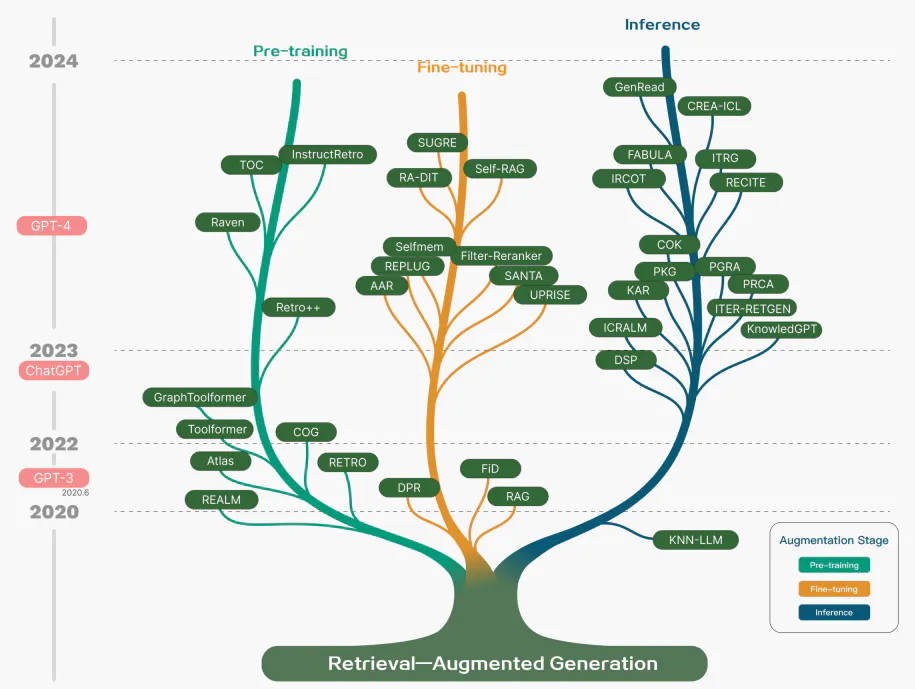
\includegraphics[width=\textwidth]{rag-tree.png}
    \caption{
        \it{ Technology tree of RAG research \cite{gao2024retrievalaugmented}}
    }
    \label{fig:rag-tree}
\end{figure}

\subsection{Retrieval Augmented Generation (RAG) Categories}

The RAG research paradigm is continuously evolving and can be categorized into three stages: Naive RAG, Advanced RAG, and Modular RAG, as shown in Figure \ref{fig:rag-categories}. Although RAG methods are cost-effective and outperform native LLMs, they also present several limitations. The development of Advanced RAG and Modular RAG addresses these specific shortcomings found in Naive RAG.

\subsubsection*{Naive RAG}

The Naive RAG research paradigm represents the earliest methodology, gaining prominence soon after the widespread adoption of ChatGPT. Naive RAG follows a traditional process encompassing indexing, retrieval, and generation, often described as a "Retrieve-Read" framework \cite{ma2023query}.

\begin{figure}[H]
    \centering
    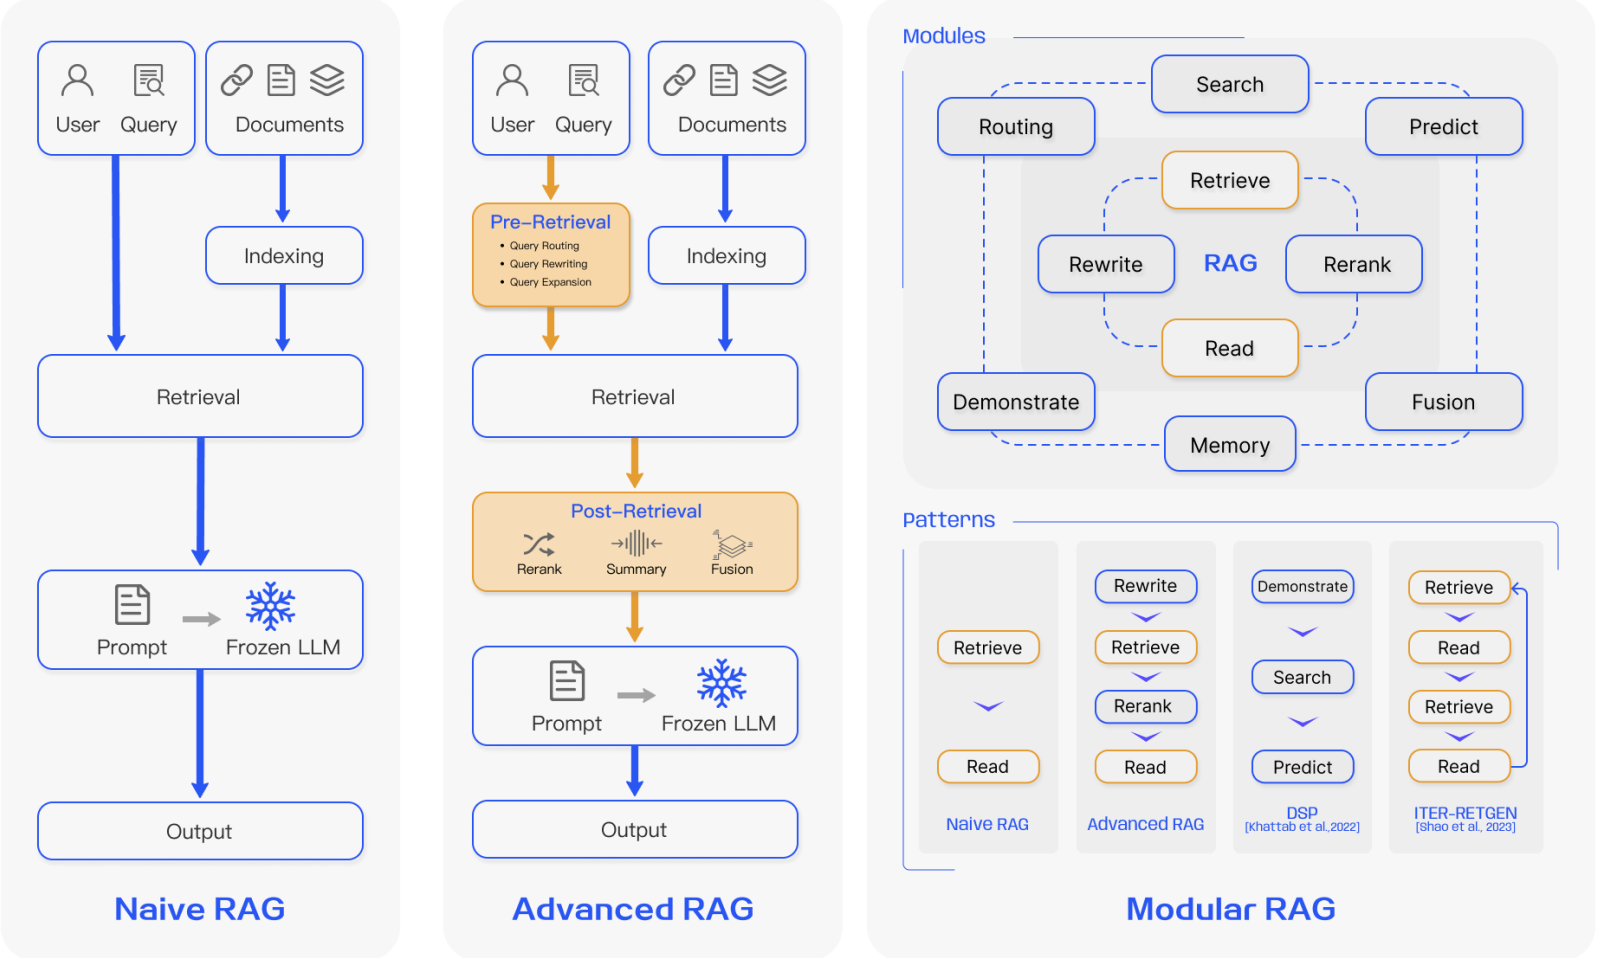
\includegraphics[width=\textwidth,height=6cm,keepaspectratio=true]{rag-categories.png}
    \caption{
        \it{ Comparison between the three paradigms of RAG \cite{gao2024retrievalaugmented}.}
    }
    \label{fig:rag-categories}
\end{figure}

Indexing starts with cleaning and extracting raw data from diverse formats like PDF, HTML, Word, and Markdown, converting it into a uniform plain text format. To address the context limitations of language models, the text is broken down into smaller, manageable chunks. These chunks are then encoded into vector representations using an embedding model and stored in a vector database. This step is critical for enabling efficient similarity searches in the next retrieval phase.

Upon receiving a user query, the RAG system employs the same encoding model used during the indexing phase to convert the query into a vector representation. It then calculates similarity scores between the query vector and the vectors of the chunks in the indexed corpus. The system prioritizes and retrieves the top K chunks that show the highest similarity to the query. These chunks are then used as the expanded context in the prompt for the generation phase.

During the generation phase, the posed query and the selected documents are combined into a coherent prompt. A large language model then formulates a response based on this prompt. The model's approach to answering can vary depending on task-specific criteria, allowing it to either utilize its inherent parametric knowledge or restrict its responses to the information within the provided documents. In cases of ongoing dialogues, any existing conversational history can be incorporated into the prompt, enabling the model to effectively engage in multi-turn interactions.

\begin{figure}[H]
    \centering
    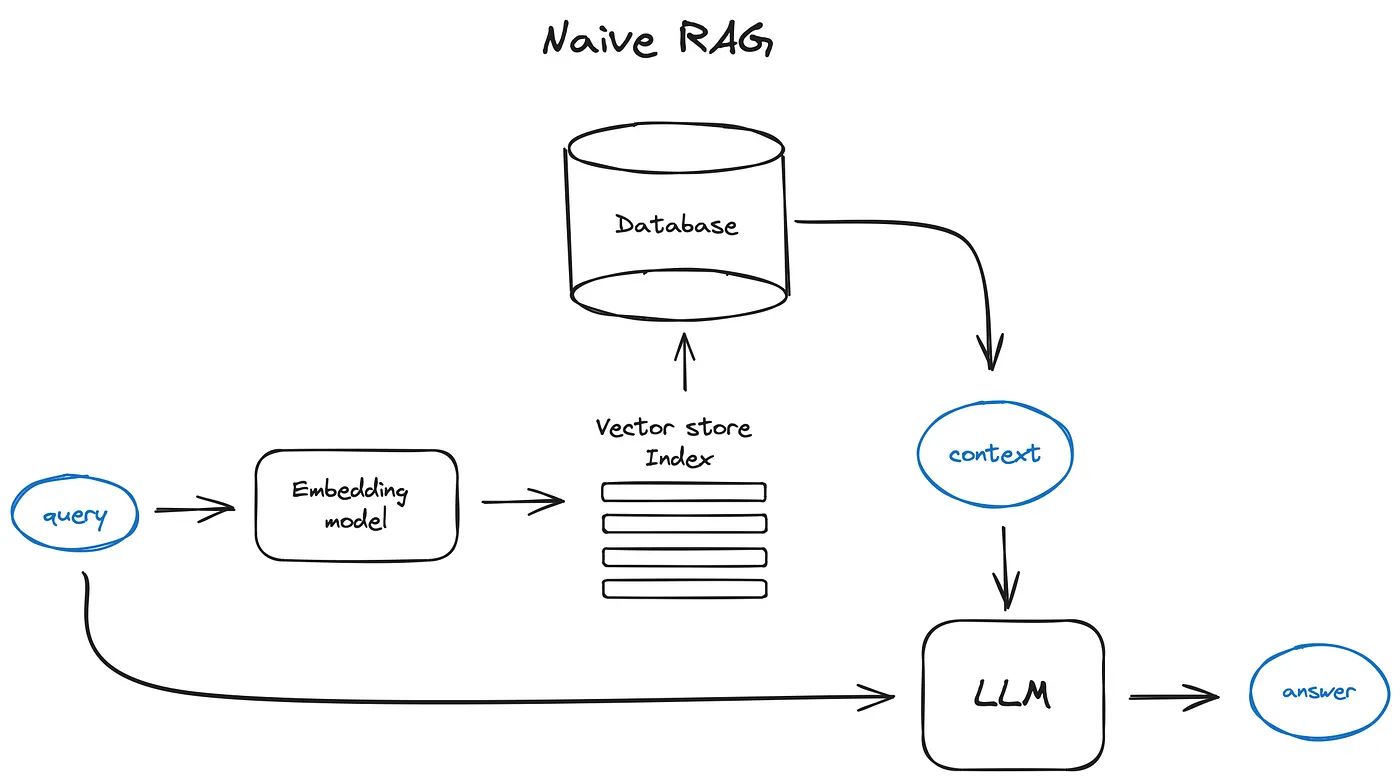
\includegraphics[width=\textwidth,height=6cm,keepaspectratio=true]{naive-rag.png}
    \caption{
        \it{Naive RAG}
    }
    \label{fig:naive-rag}
\end{figure}

\subsubsection*{Advanced RAG}

Advanced RAG introduces specific enhancements to address the limitations of Naive RAG. It focuses on improving retrieval quality through both pre-retrieval and post-retrieval strategies. To resolve indexing issues, Advanced RAG employs refined indexing techniques such as a sliding window approach, fine-grained segmentation, and the integration of metadata. Additionally, it incorporates various optimization methods to streamline the retrieval process.

\begin{figure}[H]
    \centering
    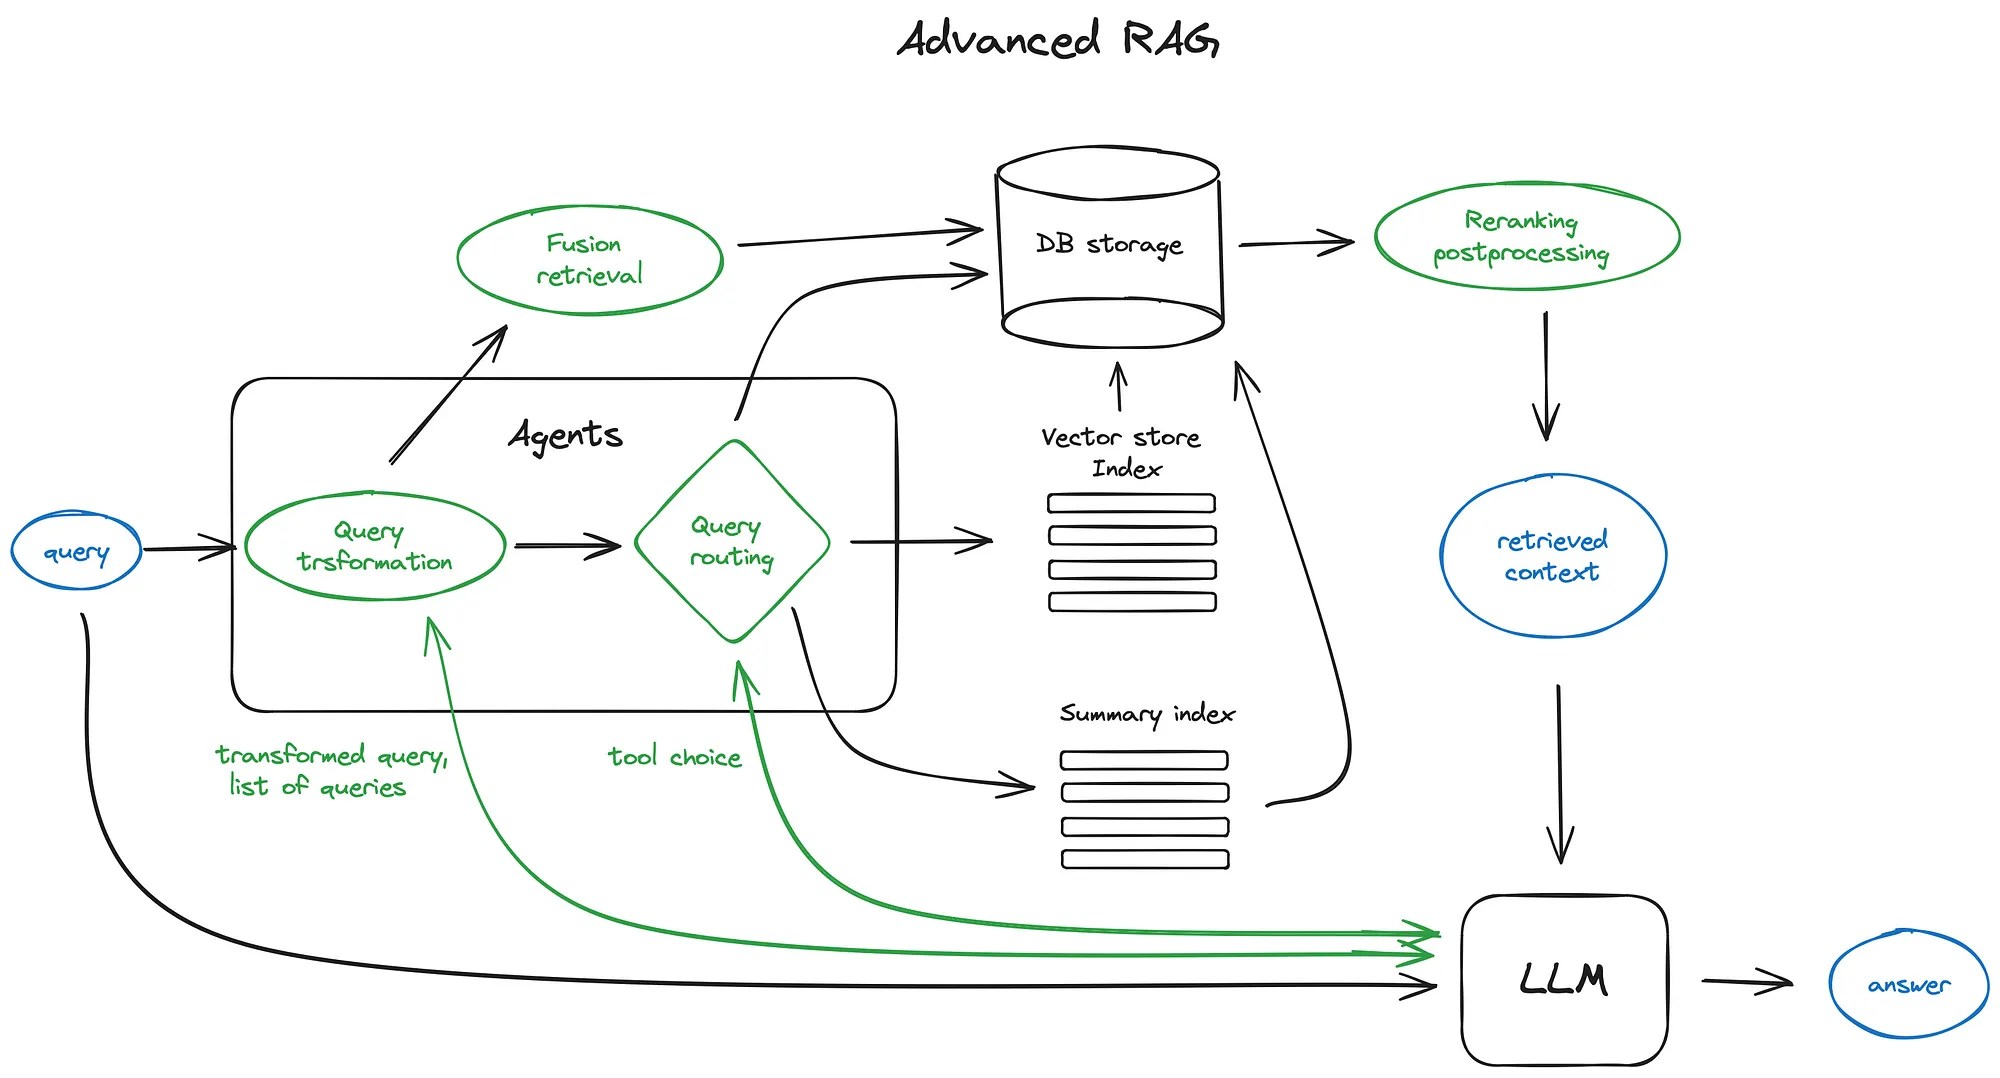
\includegraphics[width=\textwidth,height=6cm,keepaspectratio=true]{advanced-rag.png}
    \caption{
        \it{Advanced RAG}
    }
    \label{fig:advanced-rag}
\end{figure}

Pre-retrieval process. In this stage, the primary focus is on optimizing both the indexing structure and the original query. The objective of indexing optimization is to enhance the quality of the content being indexed. This involves several strategies: increasing data granularity, optimizing index structures, incorporating metadata, alignment optimization, and mixed retrieval. The goal of query optimization is to make the user's original question clearer and more suitable for retrieval. Common methods include query rewriting, query transformation, query expansion, and other techniques \cite{ma2023query}, \cite{peng2024large} \cite{gao2022precise}.

Post-Retrieval Process. Once relevant context is retrieved, it is crucial to integrate it effectively with the query. The main methods in the post-retrieval process include reranking chunks and compressing the context. Re-ranking involves adjusting the order of the retrieved information to ensure the most relevant content is positioned at the forefront of the prompt. This strategy is implemented in frameworks such as LlamaIndex\footnote{\url{https://www.llamaindex.ai/}}, LangChain\footnote{\url{https://www.langchain.com/}}, and HayStack\footnote{\url{https://haystack.deepset.ai/}}. Directly feeding all relevant documents into LLMs can cause information overload, diluting the focus on key details with irrelevant content. To mitigate this, post-retrieval efforts concentrate on selecting essential information, highlighting critical sections, and reducing the context to a manageable size for processing.

\subsubsection*{Modular RAG}

The modular RAG architecture advances beyond the earlier RAG paradigms, providing enhanced adaptability and versatility. It incorporates various strategies to improve its components, such as adding a search module for similarity searches and fine-tuning the retriever. Innovations like restructured RAG modules \cite{yu2023generate} and rearranged RAG pipelines \cite{shao2023enhancing} have been developed to address specific challenges. The trend towards a modular RAG approach is becoming increasingly common, supporting both sequential processing and integrated end-to-end training across its components. Despite its distinctiveness, Modular RAG builds on the foundational principles of Advanced and Naive RAG, demonstrating a progression and refinement within the RAG family.